\chapter[Referencial Tecnológico]{Referencial Tecnológico}
\addcontentsline{toc}{chapter}{Referencial Tecnológico}
\label{chap:tecnologico}

Neste capítulo, serão apresentadas as principais ferramentas e tecnologias que estão sendo utilizadas para elaboração, condução, desenvolvimento e análise do trabalho como um todo. Começando pelas principais ferramentas, as quais viabilizam o desenvolvimento e a análise do projeto, \hyperref[sec:principal]{Ferramentas Associadas ao projeto}, tem-se que: o versionamento/hospedagem com uso do GitHub; 

Entretanto, ainda existem outros apoios tecnológicos de relevâncias, e que merecem ser destacados. Em \hyperref[sec:demais]{Outros Apoios Tecnológicos}, há destaque para Ferramentas de Comunicação (ex. Teams e Whatsapp); e Ferramentas de Escrita da Monografia 
(ex. Latex e Overleaf).

\section{Ferramentas Associadas ao Projeto}
\label{sec:principal}

Seguem as principais ferramentas que serão consumidas para viabilizar o desenvolvimento e a análise do projeto.

\subsection{Python}

\begin{figure}[ht]
    \centering
    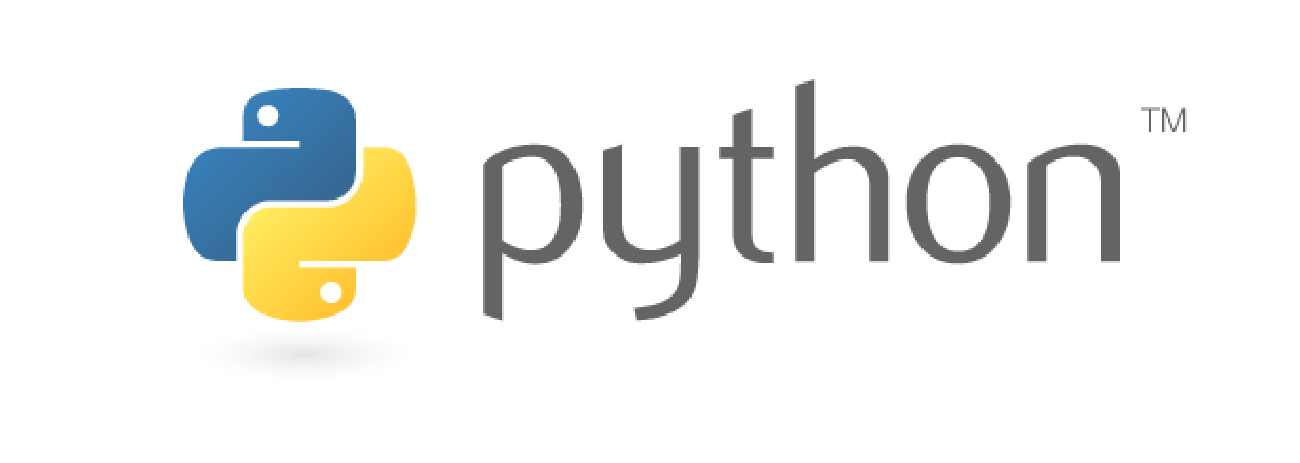
\includegraphics[scale=0.25]{figuras/referencialTecnologico/python.eps}
    \caption{Logo Python}
    \label{fig:python}
\end{figure}

Python é uma linguagem de programação de alto nível, interpretada e de propósito geral, conhecida por sua simplicidade e legibilidade. Criada por Guido van Rossum, Ela foi concebida com ênfase na facilidade de uso e na capacidade de expressar ideias de forma concisa. Seu design modular e sintaxe clara a torna uma escolha popular tanto para iniciantes quanto para desenvolvedores experientes. A filosofia central de Python, conhecida como "Zen of Python," destaca princípios como clareza, simplicidade e praticidade, guiando o desenvolvimento da linguagem.

A linguagem suporta diversos paradigmas de programação, sendo mais notavelmente associado à programação orientada a objetos. No entanto, a linguagem é multifacetada, permitindo abordagens imperativas, funcionais e procedural. Essa flexibilidade permite aos desenvolvedores escolherem o paradigma que melhor se adapta ao problema em questão, contribuindo para a versatilidade da linguagem em diferentes contextos de desenvolvimento.

Em relação aos seus prós, Python é reconhecido pela sua legibilidade e sintaxe limpa, fatores que facilitam a manutenção e colaboração em projetos. A vasta biblioteca padrão e a extensa comunidade de desenvolvedores oferecem suporte para uma ampla gama de tarefas, desde desenvolvimento web até análise de dados.

A sintaxe clara e a legibilidade do Python tornam o desenvolvimento de algoritmos de IA mais acessível, permitindo que os desenvolvedores foquem na lógica e nos conceitos subjacentes, em vez de se perderem em detalhes complexos de implementação. Além disso, a vasta biblioteca padrão e o ecossistema robusto de bibliotecas de terceiros, como NumPy, Pandas e Scikit-learn, oferecem ferramentas poderosas para manipulação de dados, processamento matemático e implementação eficiente de algoritmos de aprendizado de máquina.

Outro ponto crucial é a popularidade e o suporte contínuo que Python recebe na comunidade de ciência de dados e IA. A abundância de frameworks e bibliotecas especializadas, como TensorFlow, PyTorch e scikit-learn, todos com interfaces amigáveis, consolida a posição da linguagem como uma escolha estratégica para desenvolvedores e pesquisadores em IA. A combinação de acessibilidade, riqueza de ferramentas e apoio da comunidade faz de Python uma linguagem ideal para a concepção, prototipagem e implementação eficiente de soluções de inteligência artificial.

\subsection{TensorFlow}

\begin{figure}[ht]
	\centering
	\includegraphics[scale=0.05]{figuras/referencialTecnologico/tensorflow.eps}
	\caption{Logo TensorFlow}
	\label{fig:tensorflow}
\end{figure}

TensorFlow é uma poderosa biblioteca de código aberto desenvolvida pelo Google, projetada para facilitar a implementação de algoritmos de aprendizado de máquina e redes neurais. Destaca-se como uma das ferramentas mais populares e abrangentes no campo da inteligência artificial (IA) e aprendizado de máquina (ML). Seu nome deriva da estrutura subjacente de dados que representa fluxos multidimensionais, essenciais para operações matemáticas eficientes, fundamentais no contexto do aprendizado profundo.

A principal força do TensorFlow reside em sua flexibilidade e suporte para diversas plataformas, possibilitando o desenvolvimento e treinamento de modelos em diferentes ambientes, desde dispositivos móveis até sistemas distribuídos em larga escala. Adotando uma abordagem simbólica, o TensorFlow permite que os desenvolvedores definam e otimizem modelos complexos de maneira eficiente, com ênfase especial em redes neurais profundas. Essa flexibilidade é complementada por uma comunidade ativa e uma vasta documentação, facilitando a curva de aprendizado para novos usuários.

Entre os pontos positivos do TensorFlow, destaca-se a sua escalabilidade e eficácia no treinamento de modelos em grandes conjuntos de dados. Sua integração com unidades de processamento gráfico (GPUs) e unidades de processamento tensorial (TPUs) acelera o processamento, tornando-o ideal para projetos de aprendizado profundo.

\subsection{Keras}

Keras é uma poderosa API de alto nível projetada para simplificar o desenvolvimento de modelos de redes neurais, integrando-se perfeitamente ao TensorFlow, sendo frequentemente utilizada em conjunto com essa biblioteca. Criada com o objetivo de tornar o desenvolvimento de modelos de aprendizado profundo mais acessível, Keras oferece uma interface intuitiva e amigável, que abstrai grande parte da complexidade inerente ao aprendizado de máquina, permitindo que desenvolvedores e pesquisadores criem, treinem e testem modelos de forma rápida e eficiente.

Keras desempenha um papel de facilitar a criação e a customização de redes neurais que podem ser adaptadas tanto para o treinamento centralizado quanto para o treinamento distribuído. Sua integração com o \textit{TensorFlow Federated} permite que modelos Keras sejam aplicados em ambientes federados, onde o aprendizado ocorre de maneira descentralizada, mantendo a privacidade dos dados. Isso é particularmente relevante para o treinamento de modelos em sistemas de dados distribuídos, como em cenários onde os dados sensíveis são mantidos nos dispositivos dos usuários.

A simplicidade e modularidade do Keras o tornam uma ferramenta ideal para quem está começando no aprendizado de máquina, ao mesmo tempo em que oferece flexibilidade suficiente para projetos mais avançados. A API permite a construção rápida de modelos sequenciais e funcionais, suportando camadas como convolucionais, totalmente conectadas e recorrentes, as quais são essenciais para resolver problemas complexos em visão computacional, processamento de linguagem natural e outras áreas de IA.

Além disso, Keras oferece suporte para diversas otimizações e métricas que são fundamentais para a análise de desempenho dos modelos, seja em um ambiente centralizado ou federado. Sua capacidade de compilar modelos com diferentes otimizadores e funções de perda, como o \textit{Adam} e a \textit{sparse categorical crossentropy}, permite ajustar o comportamento dos modelos conforme as necessidades específicas do experimento, como no caso do estudo comparativo entre aprendizado centralizado e federado.

Assim como o TensorFlow, o Keras também se beneficia de uma comunidade ativa, rica documentação e suporte para execução em GPUs e TPUs, tornando-o adequado tanto para ambientes de pesquisa quanto para aplicações de produção em larga escala. Isso reforça a importância de sua escolha em projetos que buscam escalabilidade e eficiência, como os que envolvem aprendizado federado, onde o objetivo é treinar modelos em dispositivos descentralizados sem comprometer a privacidade dos dados.

\subsection{Google Colab}

\begin{figure}[ht]
	\centering
	
\includegraphics[scale=0.25]{figuras/referencialTecnologico/googleColab.eps}
	\caption{Logo Google Colab}
	\label{fig:colab}
\end{figure}

O Google Colab é uma plataforma baseada em nuvem que oferece um ambiente interativo para o desenvolvimento e execução de código Python, especialmente voltado para o aprendizado de máquina e análise de dados. A ferramenta proporciona a capacidade de criar e compartilhar notebooks Jupyter, que permitem a integração de código executável, visualizações e texto descritivo em um único documento. O Google Colab é amplamente valorizado por sua acessibilidade, uma vez que não requer configuração local e oferece acesso a recursos computacionais avançados, como unidades de processamento gráfico (GPUs) e unidades de processamento tensorial (TPUs), sem custo adicional.

No contexto deste projeto, o Google Colab foi utilizado para implementar e testar o modelo de aprendizado federado. A plataforma facilitou a execução do código de maneira eficiente e a utilização de GPUs para acelerar o treinamento do modelo, o que foi crucial para lidar com a complexidade do aprendizado federado e o processamento de grandes conjuntos de dados. Além disso, o Google Colab permitiu a documentação do progresso por meio de notebooks, que incluíram não apenas o código e os resultados das execuções, mas também as análises e visualizações das métricas de desempenho do modelo. A possibilidade de compartilhar facilmente os notebooks com os orientadores e colegas foi um aspecto importante para a colaboração e revisão contínua do projeto.

\subsection{Base de dados MNIST}

\begin{figure}[ht]
	\centering
	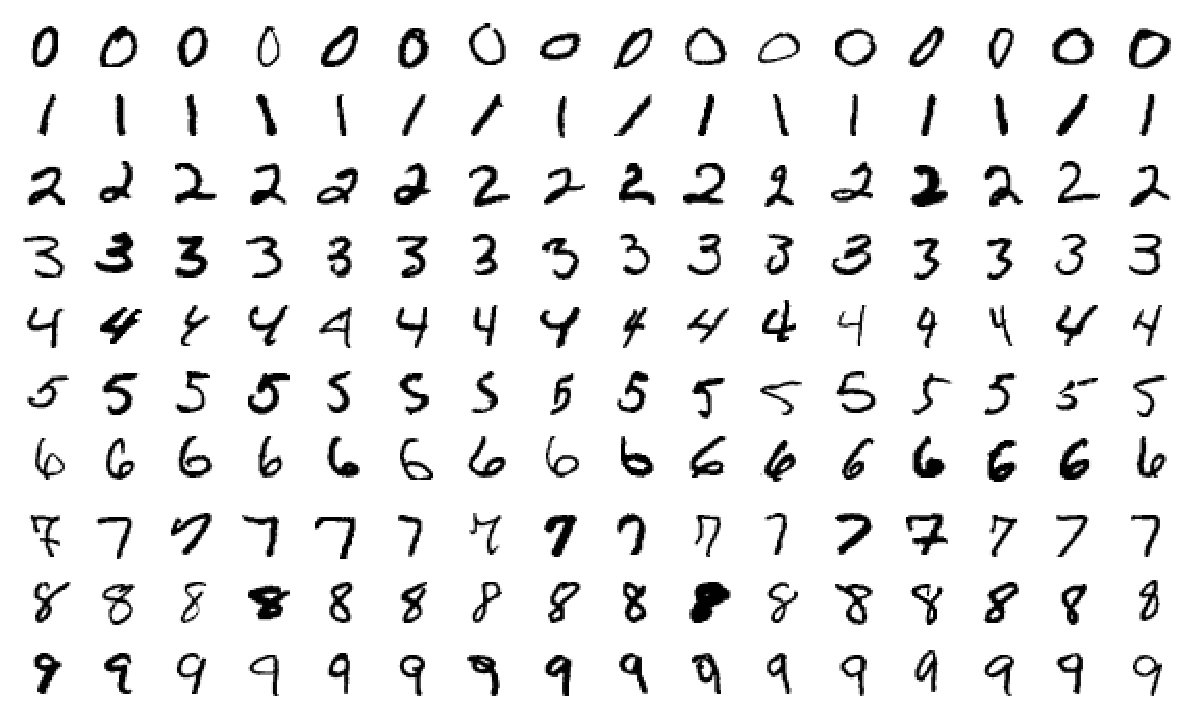
\includegraphics[scale=0.25]{figuras/referencialTecnologico/mnist.eps}
	\caption{MNIST exemplo de dados}
	\label{fig:mnist}
\end{figure}

A base de dados MNIST (Modified National Institute of Standards and Technology) é uma coleção amplamente utilizada de imagens de dígitos manuscritos que serve como um benchmark padrão para o treinamento e avaliação de algoritmos de aprendizado de máquina e redes neurais. Composta por 60.000 imagens de treinamento e 10.000 imagens de teste, cada imagem é uma matriz de 28x28 pixels em escala de cinza, representando um dígito de 0 a 9. Esta base de dados é ideal para testar modelos de classificação e redes neurais devido à sua simplicidade e ao tamanho relativamente pequeno dos dados, o que facilita a experimentação e a validação rápida de novas técnicas. A escolha do MNIST como base de dados é estratégica para avaliar o impacto de abordagens federadas em um cenário relativamente simples, fornecendo insights valiosos sobre a aplicabilidade e os desafios associados a essas técnicas em ambientes de dados reais e distribuídos.

\section{Outros Apoios Tecnológicos}
\label{sec:demais}

Seguem as demais ferramentas que auxiliam na na comunicação entre os envolvidos no projeto, bem como na escrita dessa monografia.

\subsection{Ferramentas de Comunicação}

Para comunicação entre autor e orientadores, durante a elaboração desse trabalho, destacam-se: 

\begin{itemize}
	\item O Microsoft Teams, para reuniões virtuais sobre o andamento do trabalho, e 
	\item O Whatsapp, para trocas de mensagens e avisos rápidos.
\end{itemize}

\subsection{Ferramentas de Escrita da Monografia}

Para escrita da monografia, destaca-ase o uso do LaTeX, sendo este uma linguagem de marcação para escrita de monografias comumente utilizada. Como principal vantagem tem-se a escrita 
em forma de texto simples, sem haver tanta preocupação com a formatação durante a escrita do texto. Adicionalmente foi utilizado o Overleaf para escrita do texto no formato LaTeX 
e organização das pastas, além de ser utilizado para compilar a monografia em formato PDF.

\subsection{GitHub}

\begin{figure}[ht]
	\centering
	
\includegraphics[scale=1]{figuras/referencialTecnologico/github.eps}
	\caption{Logo GitHub}
	\label{fig:github}
\end{figure}

O GitHub é uma plataforma amplamente utilizada para o versionamento de código e colaboração em projetos de software. Baseado no sistema de controle de versão Git, o GitHub oferece uma interface web que permite o gerenciamento de repositórios de código, acompanhamento de mudanças e coordenação entre equipes de desenvolvimento. A plataforma proporciona funcionalidades essenciais como a criação de branches para desenvolvimento paralelo, pull requests para revisão de código e issues para rastreamento de bugs e tarefas. 

No contexto desta pesquisa, o GitHub foi empregado para organizar e versionar o código-fonte desenvolvido, facilitando a colaboração e a documentação do progresso do projeto. A utilização do GitHub permitiu o controle de versões do código, a integração de novas funcionalidades e a correção de eventuais falhas de forma sistemática e rastreável. Além disso, a plataforma facilitou a colaboração e comunicação com orientadores e colegas, assegurando uma gestão eficiente do desenvolvimento do projeto e garantindo a integridade e a consistência do código ao longo das diferentes etapas do trabalho.